\documentclass[a4paper,oneside]{book}
%\usepackage[toc,page]{appendix}

\usepackage[utf8]{inputenc}
\usepackage[T1]{fontenc}
\usepackage[french]{babel}
%\usepackage[top=2.5cm, bottom=2.5cm, left=3.5cm, right=3cm]{geometry}
\addtolength{\textwidth}{3cm} % Marges moins larges
\addtolength{\oddsidemargin}{-1cm}	% Recentrage
\usepackage{hyperref} % Liens.
\hypersetup{
	pdfborder = {0 0 0},
}
\usepackage{fancyhdr} % Entêtes.
\lhead{}
\renewcommand{\footrulewidth}{0.8pt}
\pagestyle{fancy}
\usepackage{graphicx} % Images.
\usepackage{caption}

\usepackage{longtable}

\usepackage{array,multirow,makecell} % Tableaux.
\usepackage{tabularx}
\setcellgapes{1pt}
\makegapedcells
\newcolumntype{R}[1]{>{\raggedleft\arraybackslash }b{#1}}
\newcolumntype{L}[1]{>{\raggedright\arraybackslash }p{#1}}
\newcolumntype{C}[1]{>{\centering\arraybackslash }p{#1}}

\usepackage{lipsum}
\usepackage{minitoc}
\mtcselectlanguage{french}
\usepackage{titlesec} % Titres des chapitres
\titleformat{\chapter}[display]
{\centering\normalfont\huge\bfseries}
{\chaptertitlename\ \thechapter}
{20pt}
{\Huge}
%\usepackage{enumitem} % Indentation des lists
\usepackage{enumerate}

\usepackage{listings}
 
%\lstset{language=sql}

\usepackage{wallpaper} %title page background-----------------
%\ULCornerWallPaper{1}{fond.pdf}
\newcommand\BackgroundPicFront{
    \put(0,0){
        \parbox[b][\paperheight]{\paperwidth}{
            \vfill
            \centering
            
\includegraphics[width=\paperwidth - 1.2cm,height=\paperheight -1.5cm,keepaspectratio]{IMG/fond.eps}%
            \vfill
        }
    }
}%------------------------------------------------------------

\usepackage{hyperref} \usepackage{breakurl}
\usepackage{amsmath}
\usepackage{array}
\usepackage{subfig}
\usepackage{floatrow}

\newfloatcommand{capbtabbox}{table}[][\FBwidth]

\usepackage{color}

\definecolor{pblue}{rgb}{0.13,0.13,1}
\definecolor{pgreen}{rgb}{0,0.5,0}
\definecolor{pred}{rgb}{0.9,0,0}
\definecolor{pgrey}{rgb}{0.46,0.45,0.48}

\lstset{breaklines}
\lstset{language=Java,
  showspaces=false,
  showtabs=false,
  breaklines=true,
  showstringspaces=false,
  breakatwhitespace=true,
  commentstyle=\color{pgreen},
  keywordstyle=\color{pblue},
  stringstyle=\color{pred},
  basicstyle=\ttfamily,
  moredelim=[il][\textcolor{pgrey}]{$ $},
  moredelim=[is][\textcolor{pgrey}]{\%\%}{\%\%}
}





\begin{document}


\AddToShipoutPicture{\BackgroundPicFront}
%%%%%%%%%%%%%%%%%%%%%%%%%%%%%%%%%%%%%%%%%
% University Assignment Title Page 
% LaTeX Template
% Version 1.0 (27/12/12)
%
% This template has been downloaded from:
% http://www.LaTeXTemplates.com
%
% Original author:
% WikiBooks (http://en.wikibooks.org/wiki/LaTeX/Title_Creation)
%
% License:
% CC BY-NC-SA 3.0 (http://creativecommons.org/licenses/by-nc-sa/3.0/)
% 
% Instructions for using this template:
% This title page is capable of being compiled as is. This is not useful for 
% including it in another document. To do this, you have two options: 
%
% 1) Copy/paste everything between \begin{document} and \end{document} 
% starting at \begin{titlepage} and paste this into another LaTeX file where you 
% want your title page.
% OR
% 2) Remove everything outside the \begin{titlepage} and \end{titlepage} and 
% move this file to the same directory as the LaTeX file you wish to add it to. 
% Then add %%%%%%%%%%%%%%%%%%%%%%%%%%%%%%%%%%%%%%%%%
% University Assignment Title Page 
% LaTeX Template
% Version 1.0 (27/12/12)
%
% This template has been downloaded from:
% http://www.LaTeXTemplates.com
%
% Original author:
% WikiBooks (http://en.wikibooks.org/wiki/LaTeX/Title_Creation)
%
% License:
% CC BY-NC-SA 3.0 (http://creativecommons.org/licenses/by-nc-sa/3.0/)
% 
% Instructions for using this template:
% This title page is capable of being compiled as is. This is not useful for 
% including it in another document. To do this, you have two options: 
%
% 1) Copy/paste everything between \begin{document} and \end{document} 
% starting at \begin{titlepage} and paste this into another LaTeX file where you 
% want your title page.
% OR
% 2) Remove everything outside the \begin{titlepage} and \end{titlepage} and 
% move this file to the same directory as the LaTeX file you wish to add it to. 
% Then add %%%%%%%%%%%%%%%%%%%%%%%%%%%%%%%%%%%%%%%%%
% University Assignment Title Page 
% LaTeX Template
% Version 1.0 (27/12/12)
%
% This template has been downloaded from:
% http://www.LaTeXTemplates.com
%
% Original author:
% WikiBooks (http://en.wikibooks.org/wiki/LaTeX/Title_Creation)
%
% License:
% CC BY-NC-SA 3.0 (http://creativecommons.org/licenses/by-nc-sa/3.0/)
% 
% Instructions for using this template:
% This title page is capable of being compiled as is. This is not useful for 
% including it in another document. To do this, you have two options: 
%
% 1) Copy/paste everything between \begin{document} and \end{document} 
% starting at \begin{titlepage} and paste this into another LaTeX file where you 
% want your title page.
% OR
% 2) Remove everything outside the \begin{titlepage} and \end{titlepage} and 
% move this file to the same directory as the LaTeX file you wish to add it to. 
% Then add \input{./title_page_1.tex} to your LaTeX file where you want your
% title page.
%
%%%%%%%%%%%%%%%%%%%%%%%%%%%%%%%%%%%%%%%%%

%----------------------------------------------------------------------------------------
%	PACKAGES AND OTHER DOCUMENT CONFIGURATIONS
%----------------------------------------------------------------------------------------

%\documentclass[12pt]{article}

%\begin{document}

\begin{titlepage}
\newcommand{\HRule}{\rule{\linewidth}{0.5mm}} % Defines a new command for the horizontal lines, change thickness here

\center % Center everything on the page
 
%----------------------------------------------------------------------------------------
%	HEADING SECTIONS
%----------------------------------------------------------------------------------------
%\textsc{\small \textbf{R}épublique \textbf{A}lgérienne \textbf{D}émocratique et \textbf{P}opulaire}\\
%\textsc{\small \textbf{M}inistère de l'\textbf{E}nseignement \textbf{S}upérieur de la \textbf{R}echerche \textbf{S}cientifique}\\[0.5cm]
\textsc{\Large \textbf{U}niversité \textbf{D}e \textbf{L}orraine}\\[0.5cm] % Name of your university/college
%\begin{figure}



\includegraphics[scale=0.2]{IMG/logo.eps}\\[0.5cm]

\textsc{\small Faculté des Sciences}\\
\textsc{\small Département d'Informatique}\\[2cm]
%\textsc{\small Domaine : Mathématiques Informatique}\\
%\textsc{\small Filière : Informatique Académique}\\
%\textsc{\small Spécialité : Ingénierie du Logiciel et Traitement de l'Information}\\[0.5cm]
\textsc{\normalsize \textbf{Master I}}\\
\normalsize \textbf{Initiation à la recherche}\\[0.5cm]
\textsc{\normalsize \textbf{Sujet}}\\

%\textsc{\Large Major Heading}\\[0.5cm] % Major heading such as course name
%\textsc{\large Minor Heading}\\[0.5cm] % Minor heading such as course title

%----------------------------------------------------------------------------------------
%	TITLE SECTION
%----------------------------------------------------------------------------------------

\HRule \\[0.4cm]
{ \LARGE \bfseries Dessiner c'est prouver:\\ Quantomatic un logiciel graphique pour un raisonnement quantique}\\[0.4cm] % Title of your document
\HRule \\[1.5cm]
 
%----------------------------------------------------------------------------------------
%	AUTHOR SECTION
%----------------------------------------------------------------------------------------
\begin{flushleft}
\begin{minipage}{1\textwidth} % 1 was 0.4
\begin{flushleft} \large
\qquad\emph{\textbf{Réalisé par:}}\\[0.2cm]
\qquad \qquad Antoine \textsc{Baran}
\qquad \qquad Tarek \textsc{Mokhtari}\\ % Your name
\end{flushleft}
\end{minipage}\\%~
[1.5cm]
\begin{minipage}{1\textwidth}
\begin{flushleft} \large
\qquad\emph{\textbf{Encadrants:}} \\ % Soutenu le *.04.2015 devant le jury composé de:
\qquad \qquad Mr. Emmanuel \textsc{Jeandel} \qquad \textit{} \\ % Supervisor's Name
% \qquad \qquad ...
\qquad \qquad Mr. Simon \qquad \textsc{Perdrix} \\ % Supervisor's Name

\end{flushleft}
\end{minipage}\\[3cm]
\end{flushleft}

% If you don't want a supervisor, uncomment the two lines below and remove the section above
%\Large \emph{Author:}\\
%John \textsc{Smith}\\[3cm] % Your name

%----------------------------------------------------------------------------------------
%	DATE SECTION
%----------------------------------------------------------------------------------------

{\large \today}\\[2cm] % Date, change the \today to a set date if you want to be precise

%----------------------------------------------------------------------------------------
%	LOGO SECTION
%----------------------------------------------------------------------------------------

%\includegraphics{Logo}\\[1cm] % Include a department/university logo - this will require the graphicx package
 
%----------------------------------------------------------------------------------------

\vfill % Fill the rest of the page with whitespace
\end{titlepage}
 to your LaTeX file where you want your
% title page.
%
%%%%%%%%%%%%%%%%%%%%%%%%%%%%%%%%%%%%%%%%%

%----------------------------------------------------------------------------------------
%	PACKAGES AND OTHER DOCUMENT CONFIGURATIONS
%----------------------------------------------------------------------------------------

%\documentclass[12pt]{article}

%\begin{document}

\begin{titlepage}
\newcommand{\HRule}{\rule{\linewidth}{0.5mm}} % Defines a new command for the horizontal lines, change thickness here

\center % Center everything on the page
 
%----------------------------------------------------------------------------------------
%	HEADING SECTIONS
%----------------------------------------------------------------------------------------
%\textsc{\small \textbf{R}épublique \textbf{A}lgérienne \textbf{D}émocratique et \textbf{P}opulaire}\\
%\textsc{\small \textbf{M}inistère de l'\textbf{E}nseignement \textbf{S}upérieur de la \textbf{R}echerche \textbf{S}cientifique}\\[0.5cm]
\textsc{\Large \textbf{U}niversité \textbf{D}e \textbf{L}orraine}\\[0.5cm] % Name of your university/college
%\begin{figure}



\includegraphics[scale=0.2]{IMG/logo.eps}\\[0.5cm]

\textsc{\small Faculté des Sciences}\\
\textsc{\small Département d'Informatique}\\[2cm]
%\textsc{\small Domaine : Mathématiques Informatique}\\
%\textsc{\small Filière : Informatique Académique}\\
%\textsc{\small Spécialité : Ingénierie du Logiciel et Traitement de l'Information}\\[0.5cm]
\textsc{\normalsize \textbf{Master I}}\\
\normalsize \textbf{Initiation à la recherche}\\[0.5cm]
\textsc{\normalsize \textbf{Sujet}}\\

%\textsc{\Large Major Heading}\\[0.5cm] % Major heading such as course name
%\textsc{\large Minor Heading}\\[0.5cm] % Minor heading such as course title

%----------------------------------------------------------------------------------------
%	TITLE SECTION
%----------------------------------------------------------------------------------------

\HRule \\[0.4cm]
{ \LARGE \bfseries Dessiner c'est prouver:\\ Quantomatic un logiciel graphique pour un raisonnement quantique}\\[0.4cm] % Title of your document
\HRule \\[1.5cm]
 
%----------------------------------------------------------------------------------------
%	AUTHOR SECTION
%----------------------------------------------------------------------------------------
\begin{flushleft}
\begin{minipage}{1\textwidth} % 1 was 0.4
\begin{flushleft} \large
\qquad\emph{\textbf{Réalisé par:}}\\[0.2cm]
\qquad \qquad Antoine \textsc{Baran}
\qquad \qquad Tarek \textsc{Mokhtari}\\ % Your name
\end{flushleft}
\end{minipage}\\%~
[1.5cm]
\begin{minipage}{1\textwidth}
\begin{flushleft} \large
\qquad\emph{\textbf{Encadrants:}} \\ % Soutenu le *.04.2015 devant le jury composé de:
\qquad \qquad Mr. Emmanuel \textsc{Jeandel} \qquad \textit{} \\ % Supervisor's Name
% \qquad \qquad ...
\qquad \qquad Mr. Simon \qquad \textsc{Perdrix} \\ % Supervisor's Name

\end{flushleft}
\end{minipage}\\[3cm]
\end{flushleft}

% If you don't want a supervisor, uncomment the two lines below and remove the section above
%\Large \emph{Author:}\\
%John \textsc{Smith}\\[3cm] % Your name

%----------------------------------------------------------------------------------------
%	DATE SECTION
%----------------------------------------------------------------------------------------

{\large \today}\\[2cm] % Date, change the \today to a set date if you want to be precise

%----------------------------------------------------------------------------------------
%	LOGO SECTION
%----------------------------------------------------------------------------------------

%\includegraphics{Logo}\\[1cm] % Include a department/university logo - this will require the graphicx package
 
%----------------------------------------------------------------------------------------

\vfill % Fill the rest of the page with whitespace
\end{titlepage}
 to your LaTeX file where you want your
% title page.
%
%%%%%%%%%%%%%%%%%%%%%%%%%%%%%%%%%%%%%%%%%

%----------------------------------------------------------------------------------------
%	PACKAGES AND OTHER DOCUMENT CONFIGURATIONS
%----------------------------------------------------------------------------------------

%\documentclass[12pt]{article}

%\begin{document}

\begin{titlepage}
\newcommand{\HRule}{\rule{\linewidth}{0.5mm}} % Defines a new command for the horizontal lines, change thickness here

\center % Center everything on the page
 
%----------------------------------------------------------------------------------------
%	HEADING SECTIONS
%----------------------------------------------------------------------------------------
%\textsc{\small \textbf{R}épublique \textbf{A}lgérienne \textbf{D}émocratique et \textbf{P}opulaire}\\
%\textsc{\small \textbf{M}inistère de l'\textbf{E}nseignement \textbf{S}upérieur de la \textbf{R}echerche \textbf{S}cientifique}\\[0.5cm]
\textsc{\Large \textbf{U}niversité \textbf{D}e \textbf{L}orraine}\\[0.5cm] % Name of your university/college
%\begin{figure}



\includegraphics[scale=0.2]{IMG/logo.eps}\\[0.5cm]

\textsc{\small Faculté des Sciences}\\
\textsc{\small Département d'Informatique}\\[2cm]
%\textsc{\small Domaine : Mathématiques Informatique}\\
%\textsc{\small Filière : Informatique Académique}\\
%\textsc{\small Spécialité : Ingénierie du Logiciel et Traitement de l'Information}\\[0.5cm]
\textsc{\normalsize \textbf{Master I}}\\
\normalsize \textbf{Initiation à la recherche}\\[0.5cm]
\textsc{\normalsize \textbf{Sujet}}\\

%\textsc{\Large Major Heading}\\[0.5cm] % Major heading such as course name
%\textsc{\large Minor Heading}\\[0.5cm] % Minor heading such as course title

%----------------------------------------------------------------------------------------
%	TITLE SECTION
%----------------------------------------------------------------------------------------

\HRule \\[0.4cm]
{ \LARGE \bfseries Dessiner c'est prouver:\\ Quantomatic un logiciel graphique pour un raisonnement quantique}\\[0.4cm] % Title of your document
\HRule \\[1.5cm]
 
%----------------------------------------------------------------------------------------
%	AUTHOR SECTION
%----------------------------------------------------------------------------------------
\begin{flushleft}
\begin{minipage}{1\textwidth} % 1 was 0.4
\begin{flushleft} \large
\qquad\emph{\textbf{Réalisé par:}}\\[0.2cm]
\qquad \qquad Antoine \textsc{Baran}
\qquad \qquad Tarek \textsc{Mokhtari}\\ % Your name
\end{flushleft}
\end{minipage}\\%~
[1.5cm]
\begin{minipage}{1\textwidth}
\begin{flushleft} \large
\qquad\emph{\textbf{Encadrants:}} \\ % Soutenu le *.04.2015 devant le jury composé de:
\qquad \qquad Mr. Emmanuel \textsc{Jeandel} \qquad \textit{} \\ % Supervisor's Name
% \qquad \qquad ...
\qquad \qquad Mr. Simon \qquad \textsc{Perdrix} \\ % Supervisor's Name

\end{flushleft}
\end{minipage}\\[3cm]
\end{flushleft}

% If you don't want a supervisor, uncomment the two lines below and remove the section above
%\Large \emph{Author:}\\
%John \textsc{Smith}\\[3cm] % Your name

%----------------------------------------------------------------------------------------
%	DATE SECTION
%----------------------------------------------------------------------------------------

{\large \today}\\[2cm] % Date, change the \today to a set date if you want to be precise

%----------------------------------------------------------------------------------------
%	LOGO SECTION
%----------------------------------------------------------------------------------------

%\includegraphics{Logo}\\[1cm] % Include a department/university logo - this will require the graphicx package
 
%----------------------------------------------------------------------------------------

\vfill % Fill the rest of the page with whitespace
\end{titlepage}

\ClearShipoutPicture

\dominitoc
\setcounter{minitocdepth}{4}
\frontmatter
\setcounter{secnumdepth}{4}
\setcounter{tocdepth}{4}
\tableofcontents
\newpage
\renewcommand*\listfigurename{Liste des figures}
\listoffigures
%\newpage
%\listoftables
%\renewcommand{\tablename}{TABLEAU}


% for matrices:-------------------------
\makeatletter
\newcommand\xleftrightarrow[2][]{%
  \ext@arrow 9999{\longleftrightarrowfill@}{#1}{#2}}
\newcommand\longleftrightarrowfill@{%
  \arrowfill@\leftarrow\relbar\rightarrow}
\makeatother

\newcommand{\mymatrix}[1]
{\ensuremath{\left\updownarrow\vphantom{#1}\right.
\overset{\xleftrightarrow[\hphantom{#1}]{\text{\normalsize{$2^k$}}}}{#1}}}
%-----------------------------------------

\adjustmtc
\mainmatter
%-------------------------
\chapter*{Introduction}
\addcontentsline{toc}{chapter}{Introduction}
Le formalisme mathématique qui permet de calculer et de raisonner en informatique quantique – et plus généralement en mécanique quantique – est traditionnellement un calcul matriciel: les états quantiques sont représentés par des vecteurs et les évolutions par des matrices. Ces dernières années un langage graphique appelé ZX-calculus a été développé: le calcul matriciel y est remplacé par des diagrammes et une preuve consiste à transformer ces diagrammes suivant des règles graphiques.

Peut-on prouver autant de choses à l'aide de ce langage graphique qu'en utilisant des matrices ? Cette question est encore ouverte actuellement, la complétude du langage a seulement été démontrée pour des fragments de la mécanique quantique. Un logiciel appelé Quantomatic permet de construire des diagrammes du ZX-calculus sur ordinateur. Quantomatic permet également d'automatiser autant que possible l'application des transformations graphiques.

\chapter{ZX-Calculus}
\minitoc
\vspace{2cm}
Le ZX-Calculus est un langage graphique permettant de raisonner sur des systèmes et processus quantiques.

Ce langage est représenté par des graphes composés de sommets, d'arêtes et d'entrées/sorties, il existe trois types de sommets:

\newpage

\section{Les composants du langage}
\subsection{Les sommets verts}

\begin{center}
\hspace{1cm}
\begin{minipage}[c]{0.25\textwidth}
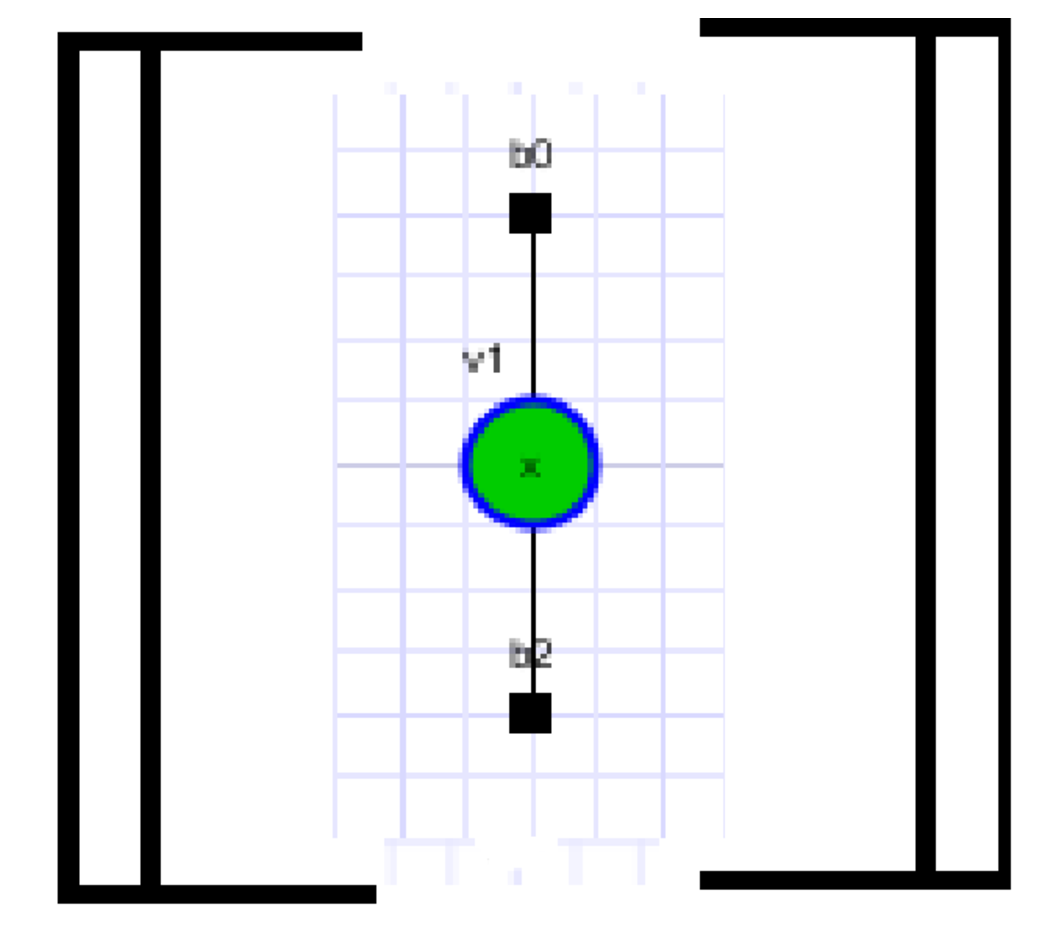
\includegraphics[scale=0.25]{IMG/sommetVert.eps}
\end{minipage}
\hspace{2cm}
\begin{minipage}[c]{0.25\textwidth}
$
\begin{pmatrix}
1 & 0 \\
0 & e^{ix}
\end{pmatrix}
$
\end{minipage}
\captionof{figure}{Un sommet vert et sa matrice correspondante.}
\label{sommetVert}
\end{center}
 
%
%

%Ici il est composé d'une entrée et d'une sortie, voici sa matrice correspondante. 
La figure \ref{sommetVert} montre un sommet vert et la matrice qui lui correspond. C'est donc une matrice toute simple sur laquelle on peut retrouver la valeur x de l'angle du sommet.

Prenons l'exemple d'un sommet vert qui a plusieurs entrées/sorties (figure \ref{sommetVertN}):

\begin{center}
\begin{minipage}[c]{0.25\textwidth}
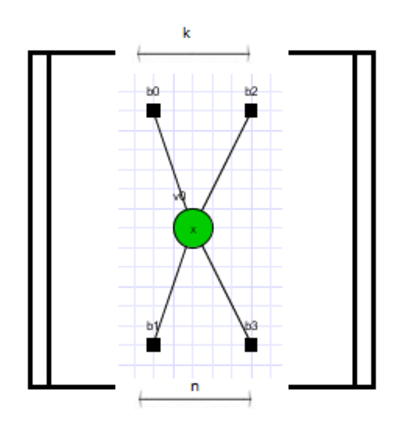
\includegraphics[scale=0.6]{IMG/sommetVertN.eps}
\end{minipage}
\hspace{1cm}
\begin{minipage}[c]{0.25\textwidth}
$
2^n
\mymatrix{\begin{pmatrix}
1 &0& \hdots & \hdots & 0 \\
0 &   &   &   & \vdots \\
\vdots  &   & \text{\Huge0}  &   & \vdots \\
\vdots  &   &   &   & 0 \\
0 & \hdots & \hdots & 0 & e^{ix} \\
\end{pmatrix}}
$
\end{minipage}
\captionof{figure}{Un sommet vert avec plusieurs E/S et sa matrice correspondante.}
\label{sommetVertN}
\end{center}

C'est presque la même matrice, sauf que le nombre d'entrées/sorties influe sur la matrice.

\subsection{Les sommets rouges}

\begin{center}
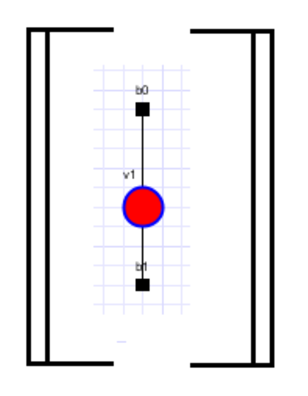
\includegraphics[scale=0.6]{IMG/sommetRouge.eps}
\captionof{figure}{Un sommet rouge.}
\label{sommetRouge}
\end{center}

La matrice d'un sommet rouge étant un peu compliquée, nous le simplifierons par le fait que c'est un sommet vert auquel on applique une transformation que nous verrons par la suite.

\subsection{Les "carrés d'Hadamard"}

\begin{center}
\hspace{1cm}
\begin{minipage}[c]{0.25\textwidth}
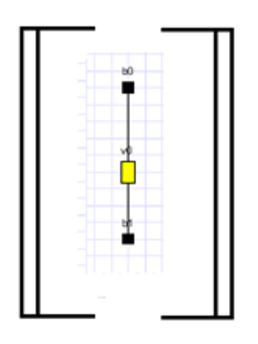
\includegraphics[scale=0.9]{IMG/hadamard.eps}
\end{minipage}
\hspace{1.5cm}
\begin{minipage}[c]{0.25\textwidth}
$
1/ \sqrt{2}
\begin{pmatrix}
1 & 1 \\
1 & -1
\end{pmatrix}
$
\end{minipage}
\captionof{figure}{Un "carré d'Hadamard" et sa matrice correspondante.}
\label{hadamrd}
\end{center}

La matrice correspondant aux carrés d'Hadamard n'est pas très compliquée non plus.

\subsection{Les arêtes}
\begin{center}
\hspace{1cm}
\begin{minipage}[c]{0.25\textwidth}
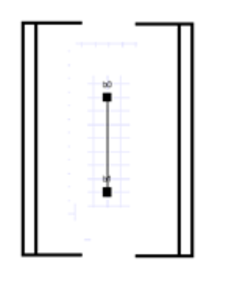
\includegraphics[scale=0.9]{IMG/arete.eps}
\end{minipage}
\hspace{1.5cm}
\begin{minipage}[c]{0.25\textwidth}
$
\begin{pmatrix}
1 & 0 \\
0 & 1
\end{pmatrix}
$
\end{minipage}
\captionof{figure}{Une arête et sa matrice correspondante.}
\label{arete}
\end{center}

La matrice d'une arête correspond simplement à la matrice identité.

\vspace{1cm}
\paragraph*{}

Comme on l'a vu, les sommets rouges et verts peuvent comporter des angles. Ces sommets peuvent être reliés par des arêtes afin de former un graphe et peuvent également comporter des « entrées-sorties ». La première partie de notre projet a donc été de nous familiariser avec ce langage graphique.

Dans le but de pouvoir faire des démonstrations dans ce langage, il existe des règles nous permettant de transformer ces graphes.

On sait que le langage est correct, si on utilise des règles de transformation sur les graphes, la matrice correspondante reste la même. C'est donc pour ça que nous allons travailler majoritairement par le biais des graphes. On remplace les calculs matriciels par des calculs graphiques.

L'objectif final de notre projet sera de savoir si, étant donné deux graphes, on peut passer de l'un à l'autre à l'aide de transformations.


\section{Matrices}
Pour parler un petit peu des matrices, voilà comment cela se présente:

\begin{center}
\begin{minipage}[c]{0.2\textwidth}
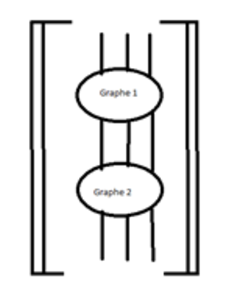
\includegraphics[scale=1]{IMG./graph21.eps}

\end{minipage}
\hspace{0.5cm}\Huge{$\longrightarrow$}
\begin{minipage}[c]{0.6\textwidth}
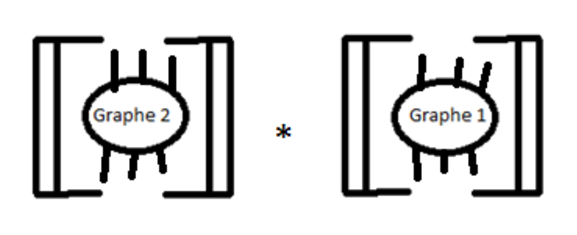
\includegraphics[scale=1]{IMG/graph2x1.eps}

\end{minipage}
\captionof{figure}{Deux graphes connectés et produit matriciel.}
\label{produitMatriciel}
\end{center}

Une matrice  qui contient deux graphes reliés peut être développé en le produit de deux matrices, l'une contenant le premier graphe et l'autre contenant le deuxième (figure \ref{produitMatriciel}.

Si par contre les deux graphes ne sont pas connectés, l'opération entre les deux matrices devient un produit tensoriel (figure \ref{produitTensoriel}):

\begin{center}
\hspace{-3cm}
\begin{minipage}[c]{0.3\textwidth}

\includegraphics[scale=0.9]{IMG./graph12.eps}
\end{minipage}
\hspace{1.5cm}\Huge{$\longrightarrow$}
\begin{minipage}[c]{0.3\textwidth}

\includegraphics[scale=0.9]{IMG/graph1x2.eps}
\end{minipage}
\captionof{figure}{Deux graphes non connectés et produit tensoriel.}
\label{produitTensoriel}
\end{center}

\subsubsection*{Exemple}
Ce qui nous donne sur un exemple simple (figure \ref{Exemple}):

\begin{center}
\centering
\begin{minipage}[c]{0.8\textwidth}
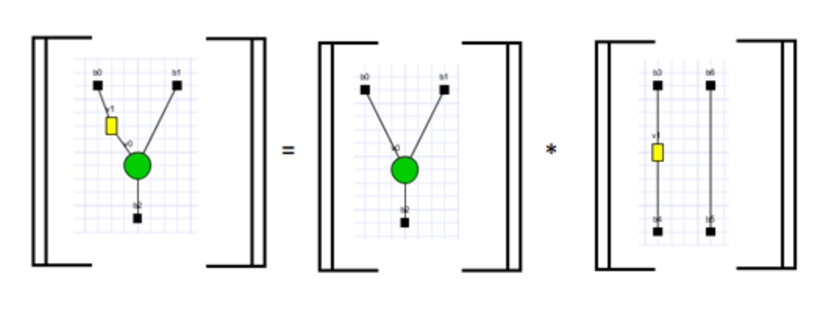
\includegraphics[scale=1]{IMG/exemple1_1.eps}
\end{minipage}
\\
\begin{minipage}[c]{0.7\textwidth}
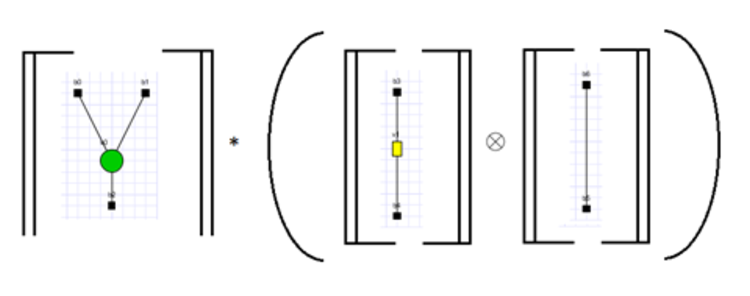
\includegraphics[scale=1]{IMG/exemple1_2.eps}
\end{minipage}
\captionof{figure}{Exemple correspondance graph $\longleftrightarrow$ matrice.}
\label{Exemple}
\end{center}

Les matrices correspondantes sont les suivantes (figure \ref{ExempleMatrices}):

\begin{center}
\begin{minipage}[c]{0.4\textwidth}
$
\begin{pmatrix}
1 & 0 & 0 & 0 \\
0 & 0 & 0 & e^{ix}
\end{pmatrix}
\begin{pmatrix}
1/ \sqrt{2}
\begin{pmatrix}
1 & 1 \\
1 & -1
\end{pmatrix} %
& \otimes & %
\begin{pmatrix}
1 & 0 \\
0 & 1
\end{pmatrix}
\end{pmatrix}
$
\end{minipage}
\captionof{figure}{Matrice correspondante à l'exemple précédent.}
\label{ExempleMatrices}
\end{center}

Mais en pratique, le but reste de pouvoir raisonner avec les diagrammes, nous allons donc voir certaines règles permettant de transformer ces diagrammes.

\section{Règles de démonstration}
\subsection{Règles de base}
Pour mieux comprendre le langage ZX-Calculus, voici les cinq premières règles sur lesquelles nous avons travaillé:

\begin{enumerate}
\item spider:\\
\begin{center}
\begin{minipage}[c]{0.25\textwidth}
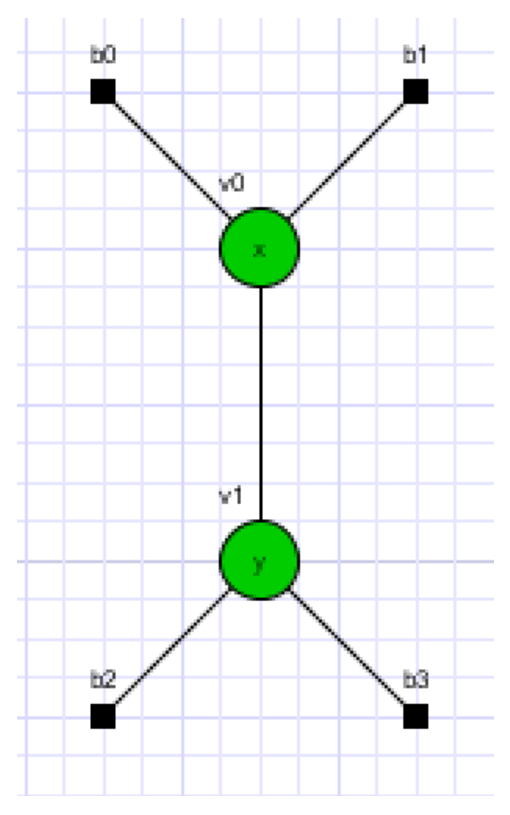
\includegraphics[scale=0.5]{IMG./spider1-2.eps}
\end{minipage}
\hspace{0.5cm}\Huge{$\longleftrightarrow$}
\begin{minipage}[c]{0.25\textwidth}
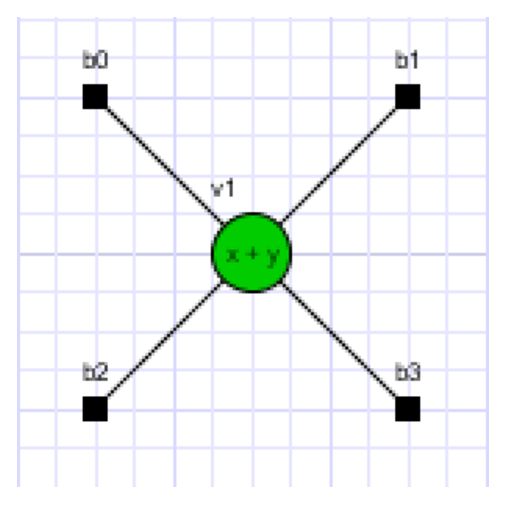
\includegraphics[scale=0.6]{IMG/spider2-2.eps}
\end{minipage}
\captionof{figure}{La règle spider.}
\label{}
\end{center}

Deux sommets de mêmes couleurs peuvent être regroupés et leurs angles sont additionnés.

\newpage

\item id:\
\begin{center}
\begin{minipage}[c]{0.25\textwidth}
\flushright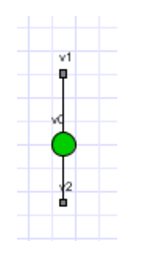
\includegraphics[scale=1]{IMG./id1.eps}
\end{minipage}
\hspace{0.5cm}\Huge{$\longleftrightarrow$}
\begin{minipage}[c]{0.25\textwidth}
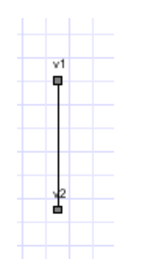
\includegraphics[scale=1]{IMG/id2.eps}
\end{minipage}
\captionof{figure}{la règle id.}
\label{id}
\end{center}

\item sp:\\
\begin{center}
\begin{minipage}[c]{0.25\textwidth}
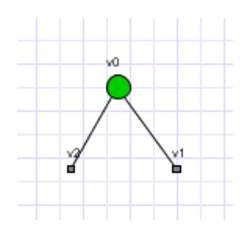
\includegraphics[scale=1]{IMG./sp1.eps}
\end{minipage}
\hspace{0.5cm}\Huge{$\longleftrightarrow$}
\begin{minipage}[c]{0.25\textwidth}
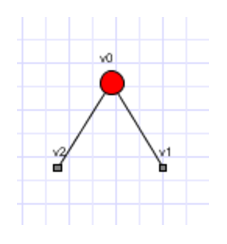
\includegraphics[scale=1]{IMG/sp2.eps}
\end{minipage}
\captionof{figure}{La règle sp.}
\label{sp}
\end{center}

\item copy:\\
\begin{center}
\begin{minipage}[c]{0.25\textwidth}
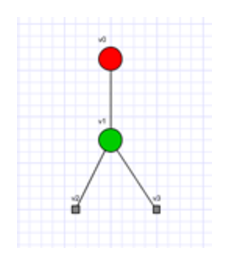
\includegraphics[scale=1]{IMG./copy1.eps}
\end{minipage}
\hspace{0.5cm}\Huge{$\longleftrightarrow$}
\begin{minipage}[c]{0.25\textwidth}
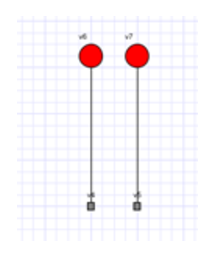
\includegraphics[scale=1]{IMG/copy2.eps}
\end{minipage}
\captionof{figure}{La règle copy.}
\label{copy}
\end{center}

\newpage

\item bialgebra:\\
\begin{center}
\begin{minipage}[c]{0.25\textwidth}
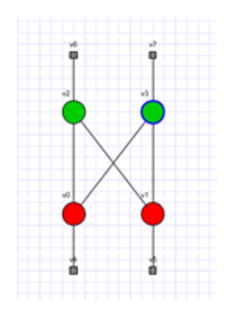
\includegraphics[scale=1]{IMG./bialgebra1.eps}
\end{minipage}
\hspace{0.5cm}\Huge{$\longleftrightarrow$}
\begin{minipage}[c]{0.25\textwidth}
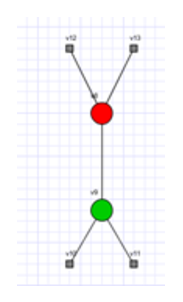
\includegraphics[scale=1]{IMG/bialgebra2.eps}
\end{minipage}
\captionof{figure}{La règle bialgebra.}
\label{bialgebra}
\end{center}
\end{enumerate}

Toutes ces règles sont possibles dans un sens comme dans l'autre, elles vont nous permettre de prouver de nouvelles règles plus complexes.

\subsection{Règles avec angles}

\begin{enumerate}
\item inversion:
\begin{center}
\begin{minipage}[c]{0.25\textwidth}
\flushright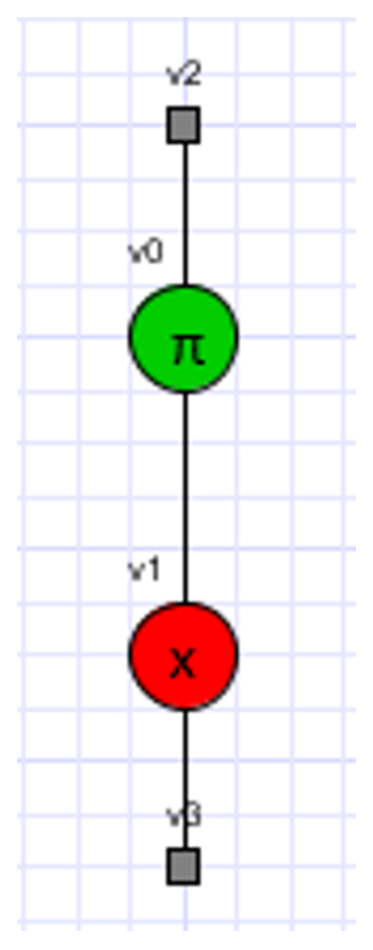
\includegraphics[scale=0.3]{IMG./inversion1-2.eps}
\end{minipage}
\hspace{0.5cm}\Huge{$\longleftrightarrow$}
\begin{minipage}[c]{0.25\textwidth}
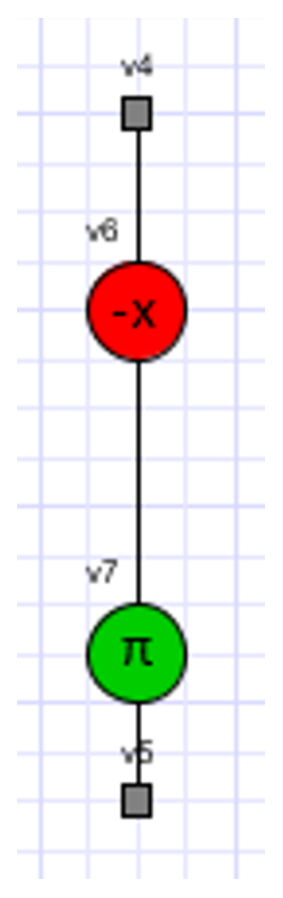
\includegraphics[scale=0.3]{IMG/inversion2-2.eps}
\end{minipage}
\captionof{figure}{La règle inversion.}
\label{inversion}
\end{center}

\item dédoublement:
\begin{center}
\begin{minipage}[c]{0.25\textwidth}
\flushright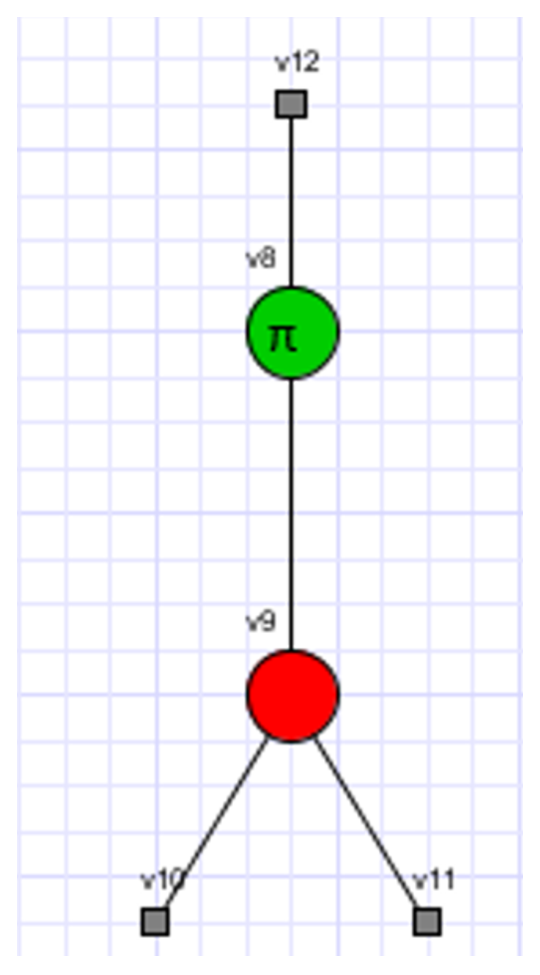
\includegraphics[scale=0.3]{IMG./dedoublement1-2.eps}
\end{minipage}
\hspace{0.5cm}\Huge{$\longleftrightarrow$}
\begin{minipage}[c]{0.25\textwidth}
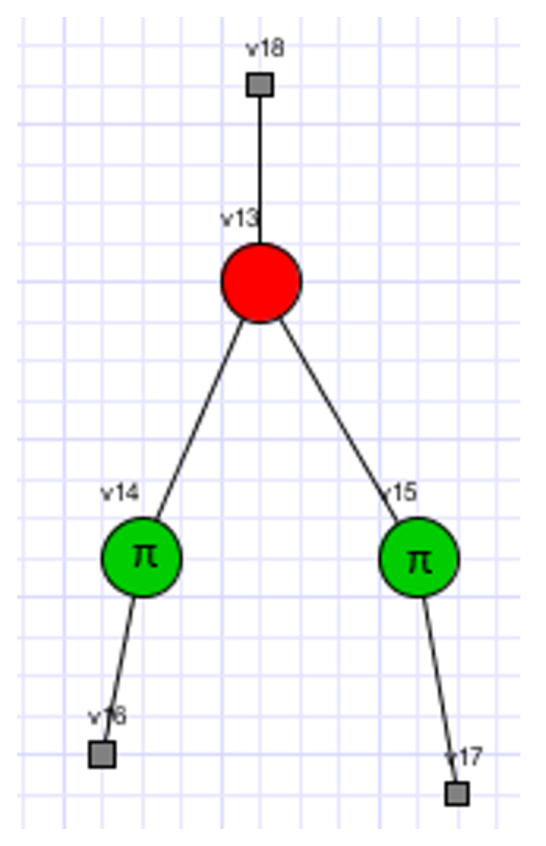
\includegraphics[scale=0.3]{IMG/dedoublement2-2.eps}
\end{minipage}
\captionof{figure}{la règle dédoublement.}
\label{dedoublement}
\end{center}

\newpage

\item changement couleur:\\
\begin{center}
\begin{minipage}[c]{0.25\textwidth}
\flushright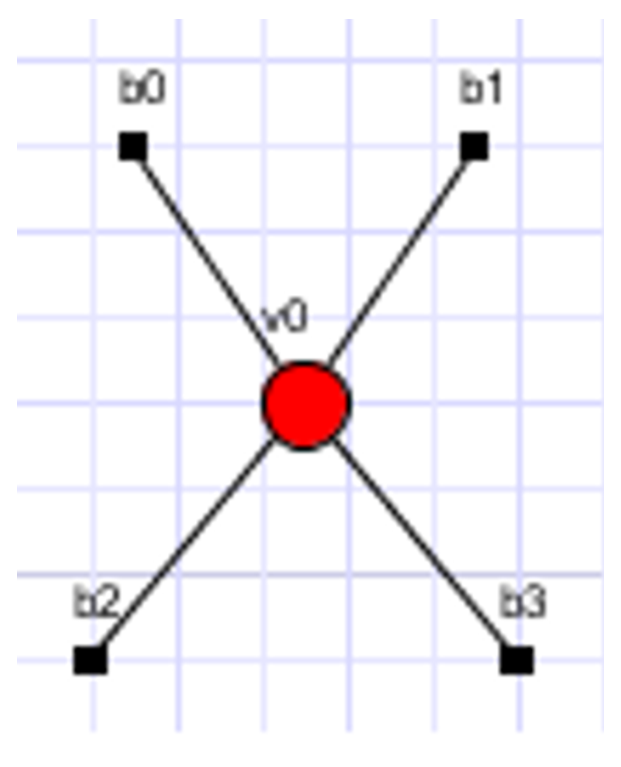
\includegraphics[scale=0.3]{IMG./changementCouleur1-2.eps}
\end{minipage}
\hspace{0.5cm}\Huge{$\longleftrightarrow$}
\begin{minipage}[c]{0.25\textwidth}
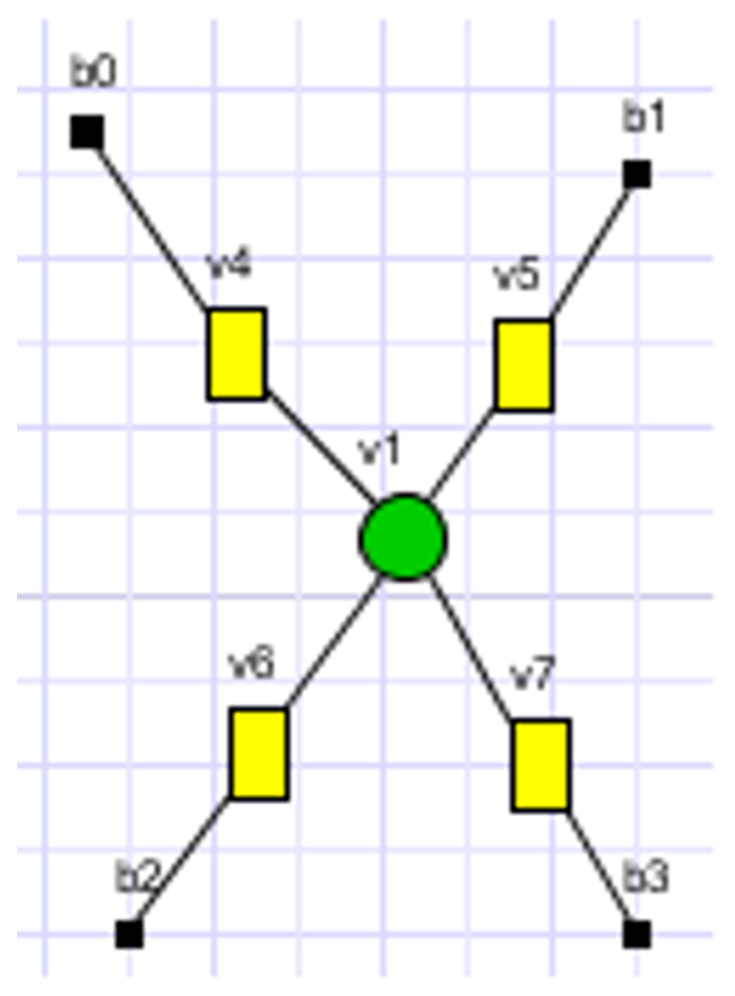
\includegraphics[scale=0.25]{IMG/changementCouleur2-2.eps}
\end{minipage}
\captionof{figure}{La règle changement couleur.}
\label{changementCouleur}
\end{center}
C'est cette dernière règle qui nous permet de calculer la matrice d'un point rouge, en transformant un sommet rouge en vert, étant donné qu'on connaît la matrice d'un carré et celle d'un sommet vert.

\item décomposition Hadamard:\\
\begin{center}
\begin{minipage}[c]{0.25\textwidth}
\flushright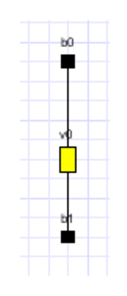
\includegraphics[scale=1]{IMG./decompositionHadamard1.eps}
\end{minipage}
\hspace{0.5cm}\Huge{$\longleftrightarrow$}
\begin{minipage}[c]{0.25\textwidth}
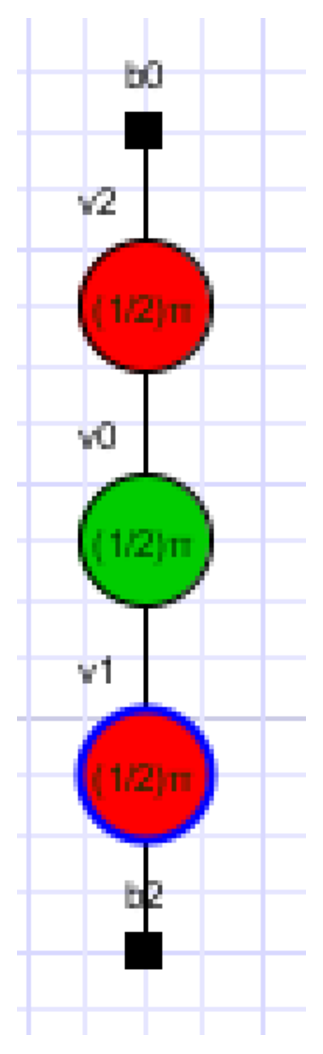
\includegraphics[scale=0.3]{IMG/decompositionHadamard2-2.eps}
\end{minipage}
\captionof{figure}{La règle décomposition Hadamard.}
\label{decompositionHadamard}
\end{center}

\item isomorphe:

Si deux graphes sont isomorphes, ils vont représenter la même matrice.

\begin{center}
\begin{minipage}[c]{0.25\textwidth}
\flushright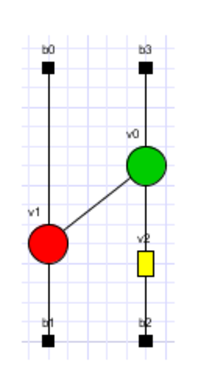
\includegraphics[scale=0.7]{IMG./isomorphe1.eps}
\end{minipage}
\hspace{0.5cm}\Huge{$\longleftrightarrow$}
\begin{minipage}[c]{0.25\textwidth}
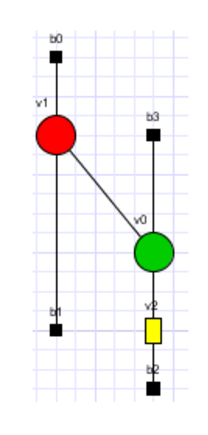
\includegraphics[scale=0.7]{IMG/isomorphe2.eps}
\end{minipage}
\captionof{figure}{La règle isomorphe.}
\label{isomorphe}
\end{center}

Ce ne sont pas les mêmes graphes mais ils gardent une même matrice, c'est une "meta-règle".

\end{enumerate}

\subsection{Démonstration}
Ces premières règles nous ont permis de prouver plusieurs nouvelles règles en partant d'un cas très simple. Au fur et à mesure des démonstrations il est possible de réutiliser les règles démontrées, de cette manière on a toujours de nouvelles possibilités pour faire des démonstrations.

Un petit exemple d'une règle que nous avons démontré (\ref{exempleDemo}) :

\begin{center}
\begin{minipage}[c]{0.2\textwidth}
\flushright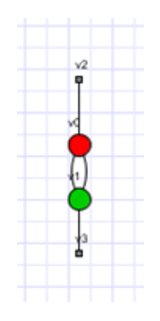
\includegraphics[scale=1]{IMG./d1.eps}
\end{minipage}
\Huge{$\longrightarrow$}
\begin{minipage}[c]{0.2\textwidth}
\flushright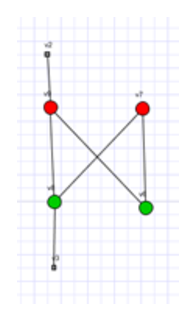
\includegraphics[scale=1]{IMG./d2.eps}
\end{minipage}
\Huge{$\longrightarrow$}
\begin{minipage}[c]{0.2\textwidth}
\flushright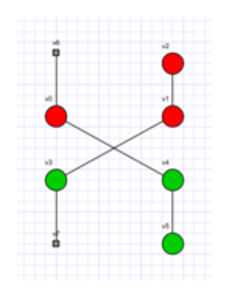
\includegraphics[scale=1]{IMG./d3.eps}
\end{minipage}
\Huge{$\longrightarrow$}
\\
\begin{minipage}[c]{0.2\textwidth}
\flushright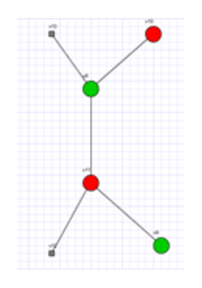
\includegraphics[scale=1]{IMG./d4.eps}
\end{minipage}
\Huge{$\longrightarrow$}
\begin{minipage}[c]{0.2\textwidth}
\flushright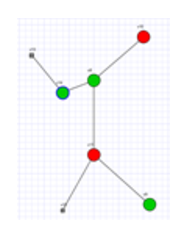
\includegraphics[scale=1]{IMG./d5.eps}
\end{minipage}
\Huge{$\longrightarrow$}
\begin{minipage}[c]{0.2\textwidth}
\flushright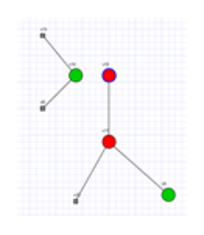
\includegraphics[scale=1]{IMG./d6.eps}
\end{minipage}
\Huge{$\longrightarrow$}
\\
\begin{minipage}[c]{0.2\textwidth}
\flushright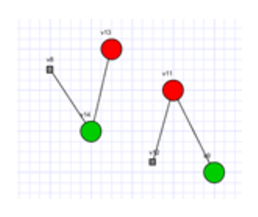
\includegraphics[scale=1]{IMG./d7.eps}
\end{minipage}
\hspace{0.7cm}\Huge{$\longrightarrow$}
\begin{minipage}[c]{0.2\textwidth}
\flushright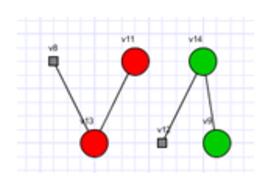
\includegraphics[scale=1]{IMG./d8.eps}
\end{minipage}
\hspace{1cm}\Huge{$\longrightarrow$}
\begin{minipage}[c]{0.2\textwidth}
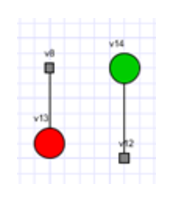
\includegraphics[scale=1]{IMG./d9.eps}
\end{minipage}

\captionof{figure}{Un exemple de démonstration d'une règle.}
\label{exempleDemo}
\end{center}

Cette démonstration nous permet maintenant de supprimer deux arêtes entre les deux mêmes sommets. Le but est donc de réussir à démontrer des règles qui vont nous faciliter d'autres dérivations.

Les règles de transformations des graphes préservent la sémantique et ne vont pas changer les matrices, les démonstrations se passent donc de la même manière, par exemple (\ref{pres}):

\begin{center}
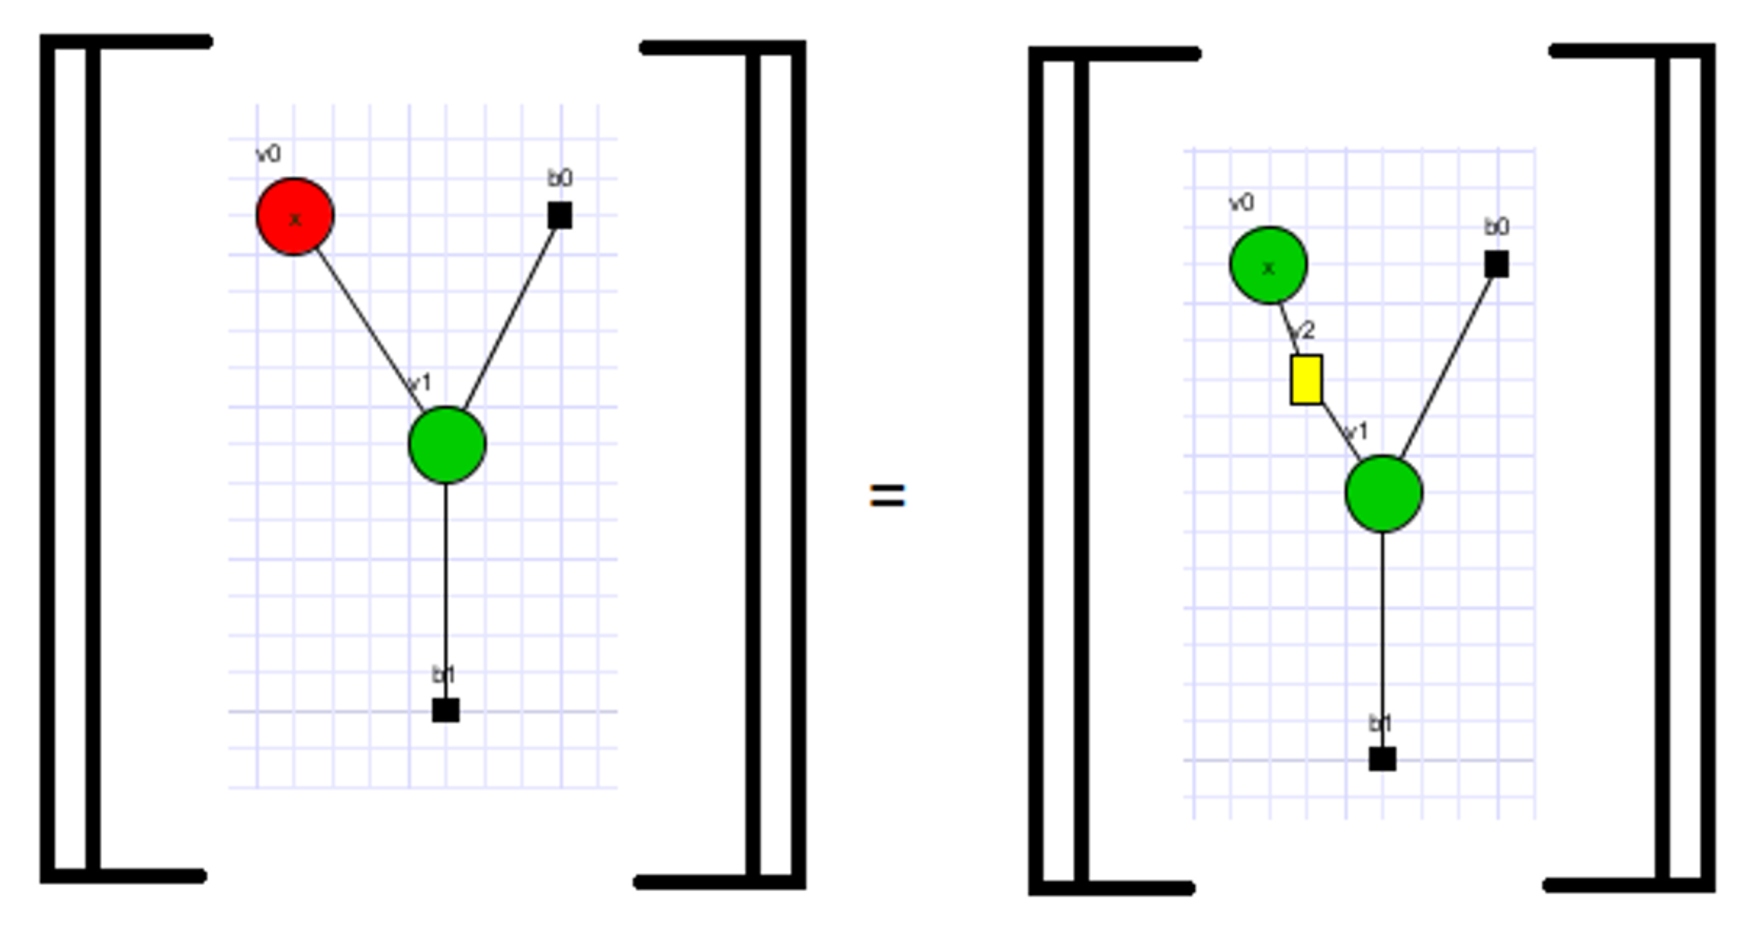
\includegraphics[scale=0.4]{IMG/pres2.eps}
\captionof{figure}{Préservation de la sémantique.}
\label{pres}
\end{center}

C'est ce qui va nous permettre de travailler principalement avec ces règles.

\section{Forme normale}
Nous cherchons à savoir si deux graphes sont égaux, pour cela on les transforme en « graph state », que nous allons définir par la suite. On veut montrer que tous les graphes peuvent se transformer en graph state.

\subsection{Parité}
Il est possible de calculer la parité (rouge ou verte) d'un graphe de la manière suivante:

\begin{center}
$P_{red}(G) \, = \,( \# Hadamards + \sum_{v \, \in \, red}^{}\sigma (v)) \, mod \, 2 $
\end{center}

La parité (ici rouge) d'un graphe est l'addition du nombre de carré d'hadamard avec la somme des degrés des sommets rouges (respectivement verts pour la parité verte), le tout modulo deux. Lors de l'application de règle à un graphe, la parité ne change en aucun cas, par exemple (\ref{parite}):

%\begin{center}
\hspace{-2.2cm}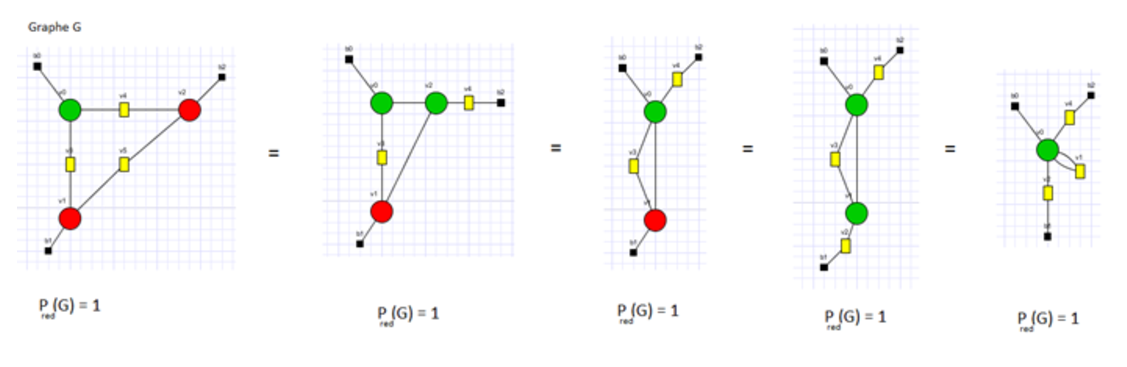
\includegraphics[scale=1]{IMG/parite.eps}
\captionof{figure}{Exemple sur la parité rouge.}
\label{parite}
%\end{center}

La parité est une condition suffisante nous permettant de dire qu'on ne peut pas passer d'un graphe D à un graphe D’. Si deux graphes n'ont pas la même parité, ils ne sont pas égaux. De cette façon c'est une petite vérification qui nous permet d'éviter de perdre du temps inutilement.

\subsection{Etat Graphe (Graph State)}
Les Etats graphes sont des graphes dont les sommets sont uniquement des sommets verts et des carrés d'Hadamard, les carrés d'Hadamard et les sommets verts ne doivent pas être reliés entre eux respectivement. En partant d'un graphe normal, le but est donc d'éliminer tous les sommets rouges et de simplifier les arrêtes "verte-verte" et "hadamard-hadamard". Le but est d'arriver à une forme sur laquelle on aime bien travailler. On aimerait trouver un ensemble de règle permettant de partir d'un graphe normal et d'arriver à son graph state.

Nous allons par la suite travailler sur ces graphs state qui sont des versions "simplifiées" des graphs normaux. Dans le cadre de notre projet les graphs state vont nous permettre de savoir plus facilement si deux graphes sont égaux, cela nous permet de ramener un problème général à un problème avec les graphs state, donc plus simple.

\chapter{Quantomatic}
\minitoc
Quantomatic est ce qu'on appelle un assistant de preuve schématique, c'est-à-dire qu'il fournit le support pour raisonner avec les langages graphiques. Quantomatic nous permet de dessiner des graphes du ZX-Calculus et y appliquer des règles de dérivation. Quantomatic a été développé par des chercheurs et des étudiants en doctorat principalement dans les universités d'Oxford et Edinburgh.

\section{Ajout théorème}
Quantomatic nous facilite la tâche lorsque nous travaillons sur le ZX-Calculus, il est possible d'ajouter de nouvelles règles pour les réutiliser par la suite. Nous partons d'un graphe simple, puis nous lui appliquons des règles de dérivation jusqu'à avoir une simplification qui nous intéresse. Nous sauvegardons ensuite la liste des règles utilisée pendant la démonstration, et à partir de cela Quantomatic nous permet d'ajouter le théorème correspondant, qui pourra maintenant être utilisé.

\section{Implémentation stratégies}
Ce Logiciel nous permet également de travailler sur des stratégies, il y a des fonctions implémentés en Poly/ML qui permettent d'appliquer une séquence de plusieurs règles dans un ordre précis à un graphe.

Nous avons donc travaillé sur ce langage pour, par exemple programmé une stratégie permettant, en partant d'un graphe, d'obtenir son "Etat graphe" grâce à une certaine séquence de règle parmi lesquels plusieurs que nous avions démontrés. Pour mieux visualiser cette stratégie, une petite illustration:

\begin{center}
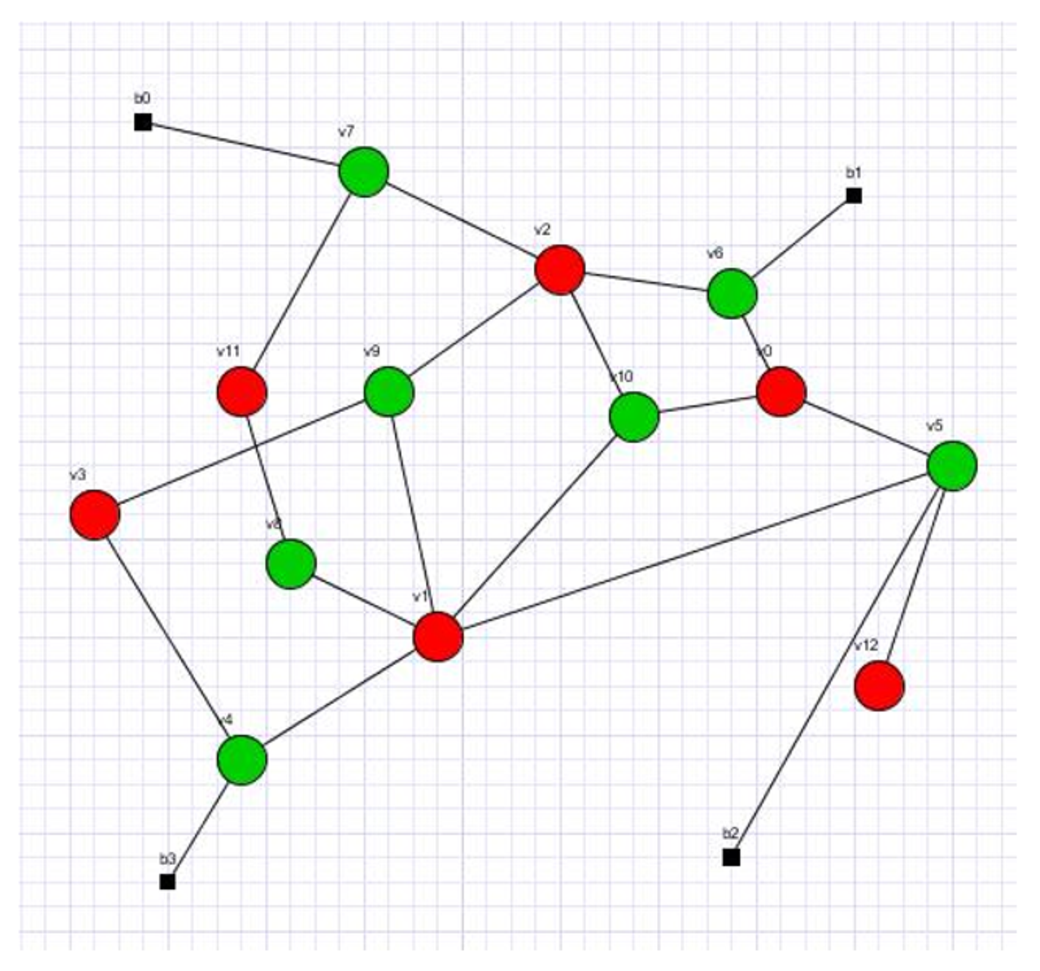
\includegraphics[scale=0.4]{IMG/strat1.eps}
\includegraphics[scale=0.4]{IMG/strat2.eps}
\includegraphics[scale=0.6]{IMG/strat3.eps}

\end{center}

La stratégie crée nous permet, à partir d'un graph de départ comme le premier, de trouver son graphe state. La liste des règles appliquées par la stratégie est décrite par la 3ème image. 

\chapter{Développement Java}
\minitoc
Le logiciel Quantomatic travaille avec des fichiers qgraph, dans le but de notre projet, nous avons  développé une petite application en java nous permettant de manipuler ces graphes et d’avoir diverse informations. Les fichiers qgraph sont écrits en Json.

\section{Informations}
A partir d'un graph venant de Quantomatic nous avons implémentés diverses fonctionnalités, il nous est possible par exemple de connaitre le nombre de sommets, de savoir quels sommets sont reliés, calculer la parité rouge ou verte d'un graphe ainsi que diverses informations concernant les angles, les voisins et les types des sommets.

\section{Manipulation}
Nous pouvons créer ou modifier un fichier qgraph qui sera manipulable par la suite dans Quantomatic en y ajoutant ou modifiant des sommets où des arêtes. Nous avons également la possibilité d'ajouté un carré d'Hadamard entre deux sommets où vérifier si un graphe donné est valide ou non, c'est-à-dire qu'il doit avoir des carrés d'Hadamard de degré 2 et des sorties de degré 1.

\section{Création (fonction "random")}
Nous avons également implémenté une fonctionnalité nous permettant de créer des graphes de manière aléatoire avec par exemple le nombre de sommets et le nombre d'entrées/sorties paramétrables. La connexion entre deux sommets est également aléatoire mais peut-être défini selon une probabilité: plus l'utilisateur choisi une probabilité élevé plus il y aura de chance d'avoir une arrête entre deux sommets.

Cette fonction nous a posé quelques problèmes puisqu'il y a plus de paramètres que ce que nous pensions à prendre en compte pour créer un graphe correcte surtout du côté des carrés d'hadamard qui sont des sommets assez spéciaux.

Etant donné que nous travaillons beaucoup sur des graphes, cela nous permet de gagner un temps considérable puisque nous n'avons plus à créer un graphe différent à chaque fois que nous voulons tester une fonctionnalité ou une stratégie sur un graphe.

Pour mieux visualiser voici un graphe \ref{random} ouvert dans Quantomatic créé par notre fonction random avec les paramètres suivants:

\begin{itemize}
\item 25 sommets.
\item 10 entrées/sorties.
\item $P_{g} = 0.3$
\item $P_{r} = 0.4 $
\item $P = 0.1 $
\end{itemize}
avec:
\begin{itemize}
\item $P_{g}$: Probabilité pour qu'un sommet soit vert lors de sa création.
\item $P_{r}$: Probabilité pour qu'un sommet soit rouge lors de sa création.
\item $P$: Lors de la génération de arêtes, en prenant les sommets (non hadamard) deux à deux, la probabilité pour que ces deux sommets soient connectés.
\end{itemize}


\begin{center}
\includegraphics[scale=0.51]{IMG/random.eps}
\captionof{figure}{Un graph généré par la fonction random.}
\label{random}
\end{center}

\newpage
\section{Concaténation}
La concaténation est une fonctionnalité que nous avons choisi d'implémenter pour assembler deux graphes. Cette fonction est exécutable de deux manières:

\subsection{Avec deux graphes en paramètre}
On prend simplement deux graphes et on les rassemble en un seul graphe sans connexion entre les deux.

\subsection{Avec deux graphes et deux entrées/sorties en paramètre}
Avec ces paramètres l'utilisateur donne deux graphes ainsi qu'une entrée/sortie du premier graphe et une entrée/sortie du deuxième graphe en paramètre. La fonction va dans ce cas assembler les deux graphes en les connectant par les entrées/sorties données en paramètre par l'utilisateur. Ce cas a été un peu plus difficile à réaliser en raison des noms des entrées/sorties qui peuvent être les mêmes pour les deux graphes. Voici une petite illustration (\ref{cat}):

\begin{center}
\begin{minipage}[c]{\textwidth}
\hspace{-1cm}\includegraphics[scale=0.5]{IMG/cat.eps}
\captionof{figure}{Un exemple de concaténation}
\label{cat}
\end{minipage}
\end{center}

On voit bien que le graphe 1 a été ajouté en haut du deuxième graphe, on y retrouve ses trois sommets.

\section{Vérification de Graphe}
Pour qu’un graphe soit correct il y a certaines vérifications  à faire : un graphe correcte est un graphe dont les carrés d'hadamard sont de degré deux et les entrées/sorties de degré un. Nous avons donc ajouté une fonctionnalité nous permettant de vérifier les graphes. Cette fonction va nous être très pratique par rapport à la création de graphe aléatoire. Du coup si on prend un cas particulier en créant un graphe avec uniquement des entrées/sorties, elles doivent toutes être reliées entre elles deux à deux. Si le nombre d'entrées/sorties est impair, c'est impossible.

\chapter*{Conclusion}
\addcontentsline{toc}{chapter}{Conclusion}
Ce projet d'initiation à la recherche nous aide donc à découvrir un peu plus comment se passe la recherche. Ici nous avons découvert entièrement un nouveau langage et travaillé dessus tout au long du semestre. Notre projet a également assez vaste puisqu'il nous a permis de manipuler à la fois les graphes sur papier, dans le logiciel Quantomatic ainsi que dans notre application en java. Malgré quelques difficultés finalement résolus, ce projet nous a plu et nous avons aimé passer du temps dessus.
\newpage
%-------------------------

\appendix
\addcontentsline{toc}{chapter}{Annexes}
\addtocontents{toc}{\protect\setcounter{tocdepth}{1}}
\makeatletter
\addtocontents{toc}{%
  \begingroup
  \let\protect\l@chapter\protect\l@section
  \let\protect\l@section\protect\l@subsection
}
\makeatother

\chapter{La fonction random}
\begin{lstlisting}[language=java]
public static QGraph random (int nVertices, int nBoundaries, double green, double red, double p) {
// Checking parameters:
if (p > 1 || p < 0) {
	System.out.println("Random: P must be between 0 and 1.");
	return null;
}
if (nVertices < 0 || nBoundaries < 0) {
	System.out.println("Random: Number of vertices and boundaries must be positif.");
	return null;
}
if (green > 1 || green < 0 || red > 1 || red < 0) {
	System.out.println("Random: parameters green (3rd) and red (4th)  must be between 0 and 1.");
	return null;
}
if (green + red > 1) {
	System.out.println("The addition of the parameters: green (3rd) and red (4th) must be inferior to 1.");
	return null;
}
if (nVertices == 0 && nBoundaries % 2 == 1) {
	System.out.println("Random: No solution for the input: (" + nVertices + "," + nBoundaries + "," + green + "," + red + "," + p + ").");
	return null;
}
if (nBoundaries % 2 == 1 && green == 0 && red == 0) {
	System.out.println("Random: No solution for the input: (" + nVertices + "," + nBoundaries + "," + green + "," + red + "," + p + ").");
	return null;
}

// Creating an empty graph: 
QGraph graph = new QGraph();

// Adding boundaries:
for (int i = 0; i < nBoundaries; i++) {
	String name = graph.addBoundary();
	graph.getBoundary(name).setX((float) (B_WIDTH * Math.cos((2 * i * Math.PI)/nBoundaries)));
	graph.getBoundary(name).setY((float) (B_HIGHT * Math.sin((2 * i * Math.PI)/nBoundaries)));
	
}

// Adding random N vertices:
double randomNumber;
for (int i = 0; i < nVertices; i++) {
	Random random = new Random();
	Random random2 = new Random();
	randomNumber  = Math.random();
	int v = random2.nextInt(5);
	String value = new String();
	switch (v) {
		case 0:
			value = new String("-\\pi");
			break;
		case 1:
			value = new String("-\\pi/2");
			break;
		case 2:
			value = new String("");
			break;
		case 3:
			value = new String("\\pi/2");
			break;
		case 4:
			value = new String("\\pi");
			break;
		default:
			break;
	}
	if (randomNumber < green) {
		//graph.addVertex(Type.GREEN);
		graph.addVertex(Type.GREEN, value, 2*MAX_X*random.nextFloat() - MAX_X, 2*MAX_Y*random.nextFloat() - MAX_Y);
	}
	else if (randomNumber < (green + red)) {
		//graph.addVertex(Type.RED);
		graph.addVertex(Type.RED, value, 2*MAX_X*random.nextFloat() - MAX_X, 2*MAX_Y*random.nextFloat() - MAX_Y);
	}
	else {
		//graph.addVertex(Type.HADAMARD);
		graph.addVertex(Type.HADAMARD, "", 2*MAX_X*random.nextFloat() - MAX_X, 2*MAX_Y*random.nextFloat() - MAX_Y);
	}
}

// Handling a special case: nBoundaries impair and all generated vertices are Hadamards:
// Change one hadamard randomly to a green or a red vertex
if (nBoundaries % 2 == 1 && nVertices > 0){
	if (graph.getNReds() + graph.getNGreens() == 0) {
		Random random = new Random();
		int r = random.nextInt(2);
		if (r == 0)
			graph.getVertex(new String ("v" + random.nextInt(nVertices))).setType(Type.GREEN);
		else if (r == 1)
			graph.getVertex(new String ("v" + random.nextInt(nVertices))).setType(Type.RED);
		
	}
}

// Handling a special case: 1 Hadamard, nothing else:
if (nVertices == 1 && !graph.getHadamards().isEmpty())
	graph.addEdge(graph.getHadamards().get(0), graph.getHadamards().get(0));
		
// Connecting boundaries to random vertices:
ArrayList<Vertex> CV;
ArrayList<Boundary> CB;

Random random = new Random();
Iterator<Boundary> iterator = graph.getBoundaries().iterator();
Boundary current;
int rand;
while (iterator.hasNext()) {
	current = iterator.next();
	CV = graph.connectableVertices();
	CB = graph.connectableBoundaries();
	
	if (graph.degree (current.getName()) > 0) {
		continue;
	}
	if (!CV.isEmpty()) {
			rand = random.nextInt(CV.size());
		graph.addEdge(current, CV.get(rand));
	}
	else {
		do {
			rand = random.nextInt(CB.size());
		} while (current.getName().equals(CB.get(rand).getName()));
		graph.addEdge(current, CB.get(rand));
	}
		
}

// Connecting Hadamards:
ArrayList<Vertex> hadamards = graph.getHadamards();
Iterator<Vertex> iterH;

for (int i = 0; i < 2; i++) {
	iterH = hadamards.iterator();
	random = new Random();
	while (iterH.hasNext()) {
		Vertex v = iterH.next();
		CV = graph.connectableVertices();
		if (graph.degree(v.getName()) == 2)
			continue;
		else {
			do {
				rand = random.nextInt(CV.size());
			} while (v.getName().equals(CV.get(rand).getName()));
			graph.addEdge(v, CV.get(rand));
		}
	}
}

// connecting other vertices according to P:
for (int i = 0; i < nVertices; i++)
	for (int j = i; j < nVertices; j++) {
		if (graph.getVertex(new String("v" + i)).getType() == Type.HADAMARD ||
			graph.getVertex(new String("v" + j)).getType() == Type.HADAMARD)
			continue;	
		else if (Math.random() < p)
			graph.addEdge(new String("v" + i), new String("v" + j));
	}
return graph;
}
\end{lstlisting}

\chapter{Stratégie permettant d'arriver vers un graph state}
\begin{lstlisting}[frame=single, language=ml]
open RG_SimpUtil

val red_elim = load_releset [
	"theorems/red_elim"
];

val simps = load_ruleset [
	"axioms/green_id", "axioms/green_sp", "theorems/double_hadamard", "theorems/par_hadamard", "axioms/copy"
];

val simplification = load_ruleset [
	"theorems/regleV", "axioms/pi0-", "axioms/greeen_hadamard2", "axioms/3pirgreen"
];

register_simproc {"strategie_red", REDUCE_ALL red_elim ++ REDUCE_ALL simps ++ REDUCE_ALL simplification ++ REDUCE_ALL simps};
\end{lstlisting}

\chapter{Quelques nouvelles règles du ZX-Calculus utilisées dans la stratégie}

\begin{enumerate}
\item regleV:
\begin{center}
\includegraphics[scale=0.5]{IMG/regleV.eps}
\end{center}

\item pi0- :
\begin{center}
\includegraphics[scale=0.5]{IMG/pi0.eps}
\end{center}

\item green\_hadamard2:
\begin{center}
\includegraphics[scale=0.5]{IMG/greenH2.eps}
\end{center}

\item 3pirgreen:
\begin{center}
\includegraphics[scale=0.45]{IMG/3pirgreen.eps}
\end{center}

\item par\_hadamard:
\begin{center}
\includegraphics[scale=0.45]{IMG/parH.eps}
\end{center}

\item double\_hadamard:
\begin{center}
\includegraphics[scale=1]{IMG/doubleH.eps}
\end{center}
\end{enumerate}

\addtocontents{toc}{\endgroup}
\backmatter
\nocite{*}
\bibliographystyle{plain} %alpha
\addcontentsline{toc}{chapter}{Références bibliographiques}
\renewcommand{\bibname}{Références bibliographiques}
\bibliography{bibliographie}
\end{document}
